\section{Introduction}
While light is massless, it imparts momenta that are significant, which: confine ion beams [\cite{Petrich1993}]; propel solar sails [\cite{Janhunen2007}]; rotate and twist objects [\cite{Beth1936, Paterson2001, Tsai2014}]; levitate, trap, and move matter [\cite{Laboratories1997, NieminenRev, Novotny1997}]; cool atoms [\cite{Weiner1999}]; and alter the crystallization of solids [\cite{Chowdhury1985}]. Our knowledge of light's momentum transfer is intrinsic to the design of facilities for low-temperature and high-energy physics, cell and molecular biology, and advanced materials research [\cite{Laboratories1997}], and is relevant to an expansive development of optomechanical devices for sensors and electronics technologies [\cite{Hugel2002, Kippenberg2007, Thourhout2010}].  Currently, the laser trapping of uncharged dielectric matter is commonplace [\cite{Laboratories1997}]; however, the optically-induced mechanics of conducting or plasmonic nanoparticles have been shown to be, at the very least, more complex [\cite{Dienerowitz2008, Saija2009, Shvedov2010, Yan2012, Yan2012a, Yan2013, Yan2013a, Yan2013b}]. One challenge stems from the numerous channels through which energy is transferred: particles also move in the presence of electric fields, magnetic fields, and thermal gradients [\cite{Bhatt, Keshoju, Edwards2006}], which are directly and indirectly produced by plasmons.  Understanding these dynamic, momentum-conserving mechanisms involves, in part, understanding the interactions among these fields.


Theoretical considerations of the gradient-intensity trapping forces, radiation pressure forces, and induced-electric-dipole interactions [\cite{Laboratories1997}] are insufficient for predicting the optomechanical behavior of plasmonic nanoparticles.  It is increasingly apparent that the excitation of plasmons play a critical role in the optically-induced movement of nonspherical nanoparticles [\cite{Yan2013}]. For example, a model of the induced electric dipole with an electric field only predicts that silver nanorods will align parallel to the direction of the illuminating linear polarization of light [\cite{Tong}], and that nanowires rotate continuously in the presence of circularly-polarized light or optical vortices via the transfer of spin or orbital angular momentum, respectively [\cite{Yan2013a, Lehmuskero1, Lehmuskero:14}]. However, this theoretical model that considers the nanoparticle polarizability alone cannot discriminate between the different mechanical behaviors associated with different nanorod-ends and particle aspect ratios [\cite{Tong}].  Nanoparticle geometry often dictates local surface plasmon modes [\cite{Knight2007}]; further insight into the physical phenomena that underlie the optomechanical behavior of non-spherical plasmonic particles is necessary.

This chapter investigates the Lorentz forces strictly attributed to surface plasmons on metal nanowires, which are of wide technological interest [\cite{Knight2007, Lal2007, Maier2005}], and potentially relevant to other plasmonic nanostructures such as carbon nanotubes, where similar chiral plasmonic behavior is tunable from the UV to THz [\cite{PhysRevBnanotube}]. The first successful trapping of a nanowire in a 3D optical trap identified an important role of plasmons. Yan, {\it et al.,} demonstrate that gold nanowires---but significantly, {\it not} silver nanowires---are confined by a Gaussian-beam optical trap [\cite{Yan2013}].  Yan proposes that the macroscopic perspective of optical trapping is insufficient and should be replaced with a plasmonic model [\cite{Yan2012}] and identifies asymmetric modes with trapping instabilities; nevertheless, a simple model that connects the dynamic instability of nanowires with its plasmonic behavior has not yet been advanced.

Plasmonically-induced Lorentz forces that are produced on gold nanowires by the illumination of linearly-polarized electromagnetic plane waves are investigated via numerical simulation.  The plasmonically-induced forces are significant in chiral geometries and when chiral hybrid plasmonic modes [\cite{Zhang2011}] are present.  This chapter identifies the electromagnetic torque and compression on the nanowires associated with the surface currents and asymmetric time-averaged fields. The results identify significant mechanical forces produced by surface plasmons in chiral hybrid modes that are currently neglected. Plasmonically-induced Lorentz forces are even expected to critically prevent the stable optical trapping of conducting nanowires, particularly when longer trapping-laser wavelengths {\it between} strong absorption resonances are employed. The approach highlights a critical dependence of nanoparticle shape [\cite{Knight2007, Tong}] and plasmon relaxation [\cite{Yan2013}] on the optically-induced forces, and considerations are relevant to future microfluidic applications.

This chapter is organized as follows. In Sec.~\ref{intro} the chiral geometry of our system is described, the numerical computations associated with Lorentz forces are outlined, and the asymmetric surface plasmon modes is illustrated. The electric dipole and plasmonic Lorentz forces of nanowires that are aligned in the transverse plane are evaluated, and agree with and clarify prior experimental results. In Sec.~\ref{forces}, the axial and translation forces associated with surface plasmons are described, these forces are generally stronger than those associated with electric dipoles.  In Sec.~\ref{3D} an analysis of the torque forces that arise from the 3D scattering is provided.  Analysis in this chapter ignores any nonlinear responses that may arise due to heat [\cite{Shvedov2010}], steam [\cite{Saija2009, Fang2013}], the electrochemical response of solvent [\cite{Arcenegui2013}], and nonlinear magneto-optical effects [\cite{Singh, Moocarme2014}], although these effects are not negligible, particularly at high illumination intensities.  Surface effects that may arise in the interaction between nanoparticles due to coatings or interfaces are also ignored, however this work is highly relevant to the understanding of such interactions with plasmonic materials [\cite{Bonin}].  The mechanical translation, compression, and torque forces associated with the plasmonic surface currents are significant and interfere with the optical trapping of elongated nanoparticles. The results in this chapter indicate that there exists a frequency cut-off at which the chiral plasmon excitation is minimized; avoiding chiral plasmon excitation will provide greater trapping stability.

\section{Setup and simulations of 2D dynamics}\label{intro}
\subsection{Calculation of electromagnetic fields}
\begin{figure}[ht]
\centering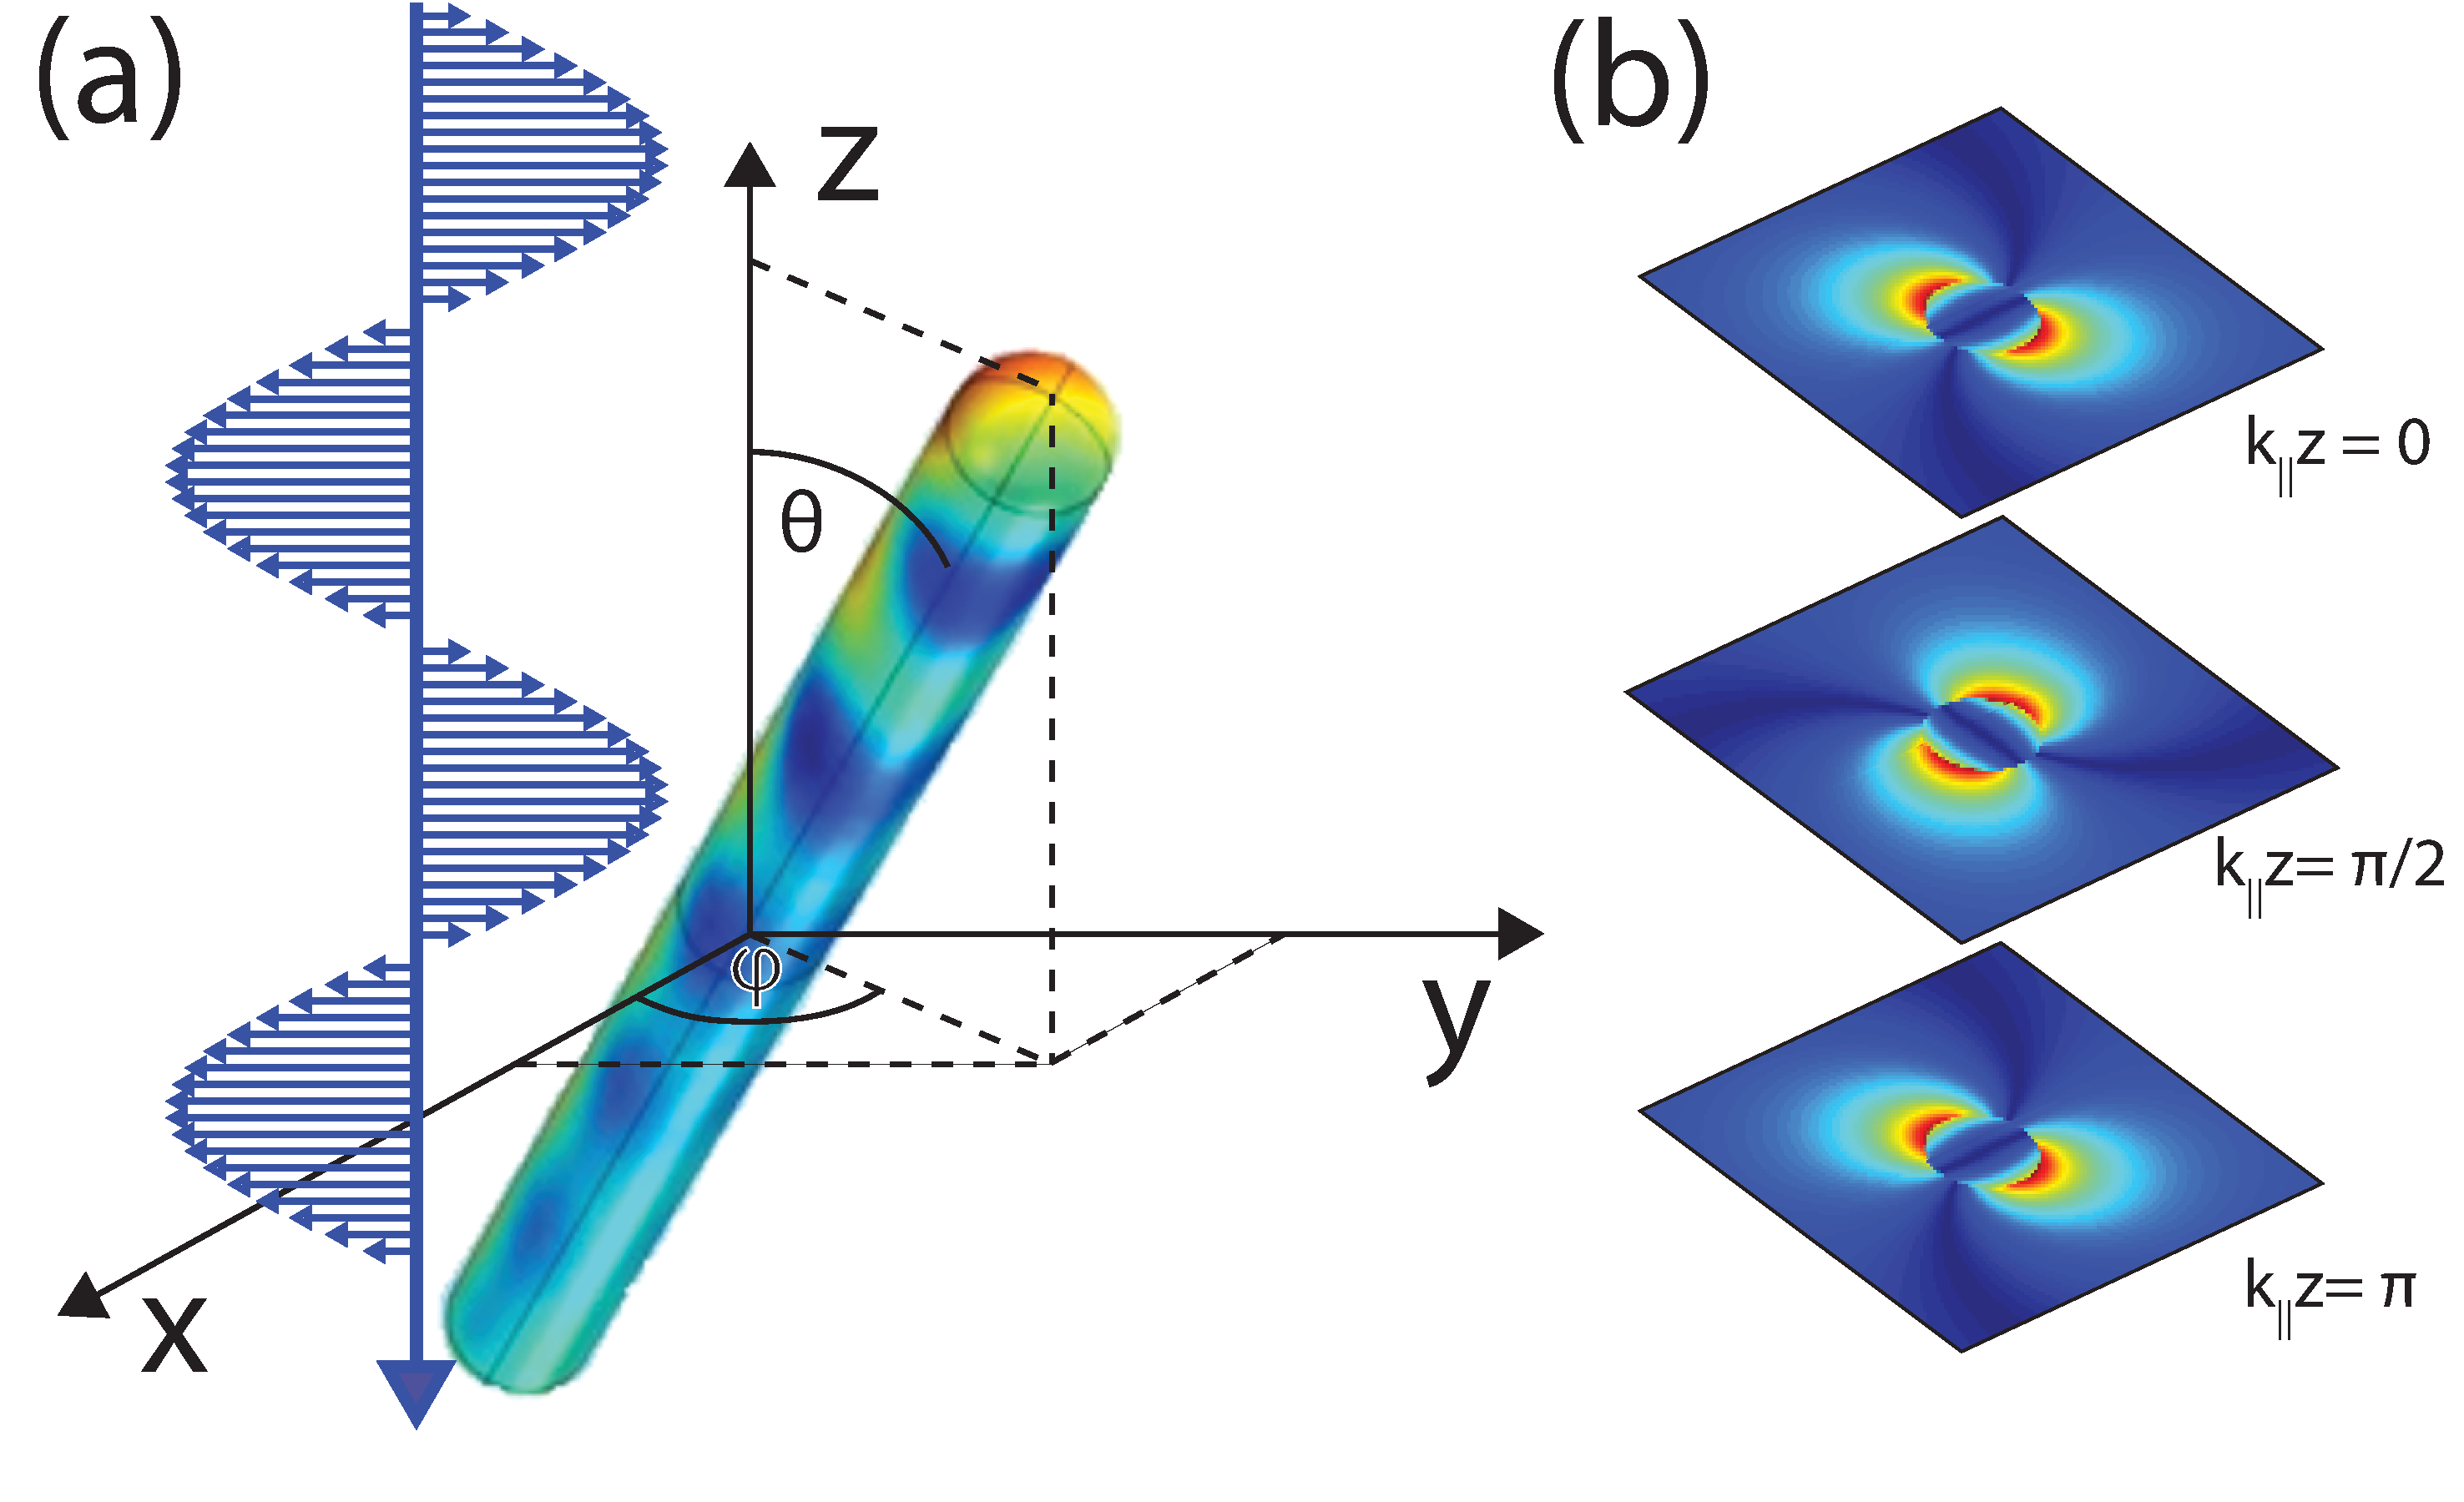
\includegraphics[width=0.95\textwidth]{SetupPicMatt.pdf}
\caption{(a) System geometry: a gold nanowire (75-nm diameter, rounded-cap, 1025-nm length) is aligned about spherical coordinates $\theta$ and $\phi$, and a $y$-polarized electromagnetic wave (1 W$/$cm$^2$) travels in the $-z$ direction. (b) The electric field profile surrounding a nanowire resulting from superposed angular momentum modes $m=0,\pm1$ with propagation lengths
$k_{\parallel}z = 0$, $\pi/2$, and $\pi$.\label{setup}}
\end{figure}

In the numerical investigation (COMSOL v4.3a, RF module, $\sim$2 million degrees of freedom), a linearly-polarized plane wave illuminates a gold nanowire immersed in deionized water, whose orientation is determined by $\theta$ and $\phi$, as illustrated in Fig. \ref{setup}(a). The nanowire dimensions are fixed with 75-nm diameter, and 950-nm length.  The nanowire terminations are hemispherical, thus the nanowire measures 1025-nm end-to-end.
%We use rounded terminations which couple the modes differently compared to flat terminations via mode-match conditions~\cite{Li2010} .
 The electromagnetic waves are polarized in the $y$-direction and propagate in the negative-$z$ direction.

In particular, this chapter focuses on the dynamics that occur when the wire is tilted towards the incoming plane wave, i.e., $\theta \neq 90^\circ$. Such arrangements produce chiral plasmons, which are superpositions of the transverse and longitudinal modes.  The signature for such modes is a time-averaged electric-field amplitude on the surface of the nanowire that varies azimuthally and over the length of the sample, a result of the superposition of two or more plasmon modes with varying azimuthal angular momentum number $m$, which are excited simultaneously by the incident fields.  The phase difference associated with the different angular momentum numbers $m$ determines the asymmetric nanowire intensity patterns [\cite{Zhang2011}]. In cylindrical coordinates the electromagnetic fields take the form [\cite{Chang2007}]:

\begin{eqnarray}\label{Efield}
E_j(r) = \frac{1}{k_j}& \sum_m&\Big\{\big[\frac{m}{s}a_{j,m}F_{j,m}+\frac{k^{(\parallel)}_{m}k^{(\perp)}_{j ,m}}{k_j}b_{j,m}F_{j,m}'\big]i\hat{s}\nonumber \\
  &-&\big[{k_{j ,m}^{(\perp)}}a_{j,m}F_{j,m}'+\frac{mk^{(\parallel)}_{m}}{k_js}b_{j,m}F_{j,m}\big]\hat{\phi} \\
  &+& \frac{[k^{(\perp)}_{j ,m}]^2}{k_j}b_{j,m}F_{j,m}\hat{z}\Big\}e^{ik^{(\parallel)}_{m}z+im\phi} \nonumber
\end{eqnarray}



\begin{eqnarray}\label{Hfield}
H_j(r) = \frac{i}{\omega\mu_0}&\sum_m &\Big\{\big[\frac{k^{(\parallel)}_{m}k_{j ,m}^{(\perp)}}{k_j}a_{j,m}F_{j,m}'+\frac{m}{s}b_{j,m}F_{j,m}\big]i\hat{s}\nonumber \\
&-&\big[\frac{mk^{(\parallel)}_{m}}{k_js}a_{j,m}F_{j,m}+{k_{j ,m}^{(\perp)}}F_{j,m}'\big]\hat{\phi}\\
&+&\frac{[k_{j ,m}^{(\perp)}]^2}{k_j}a_{j,m}F_{j,m}\hat{z}\Big\}e^{ik^{(\parallel)}_{m}z+im\phi}\nonumber
\end{eqnarray}
where $(s,\phi,z)$ are the cylindrical coordinates, the wave vectors are related by $\epsilon_jk_0^2=[k_{j ,m}^{(\perp)}]^2+[k^{(\parallel)}_m]^2$ where $\epsilon_j$ is the dielectric constant in region $j$ and $k_0$ is the wave vector in vacuum. $j=1$ outside the cylinder where $F_{1,m} = H_m (k_{1,m}^{(\perp)} s)$, the Hankel function of $m^{th}$ kind. $j=2$ inside the cylinder where $F_{2,m} = J_m(k_{2,m}^{(\perp)} s)$, the Bessel function of $m^{th}$ kind, and primes denote derivatives with respect to the argument. $a_{j,m}$ and $b_{j,m}$ are constants determined by boundary conditions. The modes excited in this system are the $m=0$, TM$_0$ mode and two degenerate first order $m=\pm 1$ modes, HE$_{\pm 1}$. Specifically, chiral-hybrid modes occur when all three of the lower order modes are simultaneously excited \textit{and} there is a phase difference between the HE$_1$ and HE$_{-1}$ modes.
A superposition of the three lowest order modes, $|m|\leq 1$ are shown in Fig. \ref{setup}(b) at different cross-sections of the nanowire corresponding to $k^{(\parallel)}_1z = 0, \pi/2$, and $\pi$. In general, the patterns in the electromagnetic fields produced off-resonance correspond to a periodic, asymmetric pattern on the wire that neither carries mirror symmetry along the length nor across the width of the wire.  It is anticipated that this asymmetry, which arises from the chiral illumination geometry, that produces a net translation and torques via Lorentz forces.

\subsection{Calculation of Lorentz force}
The well-known Lorentz law, $\mathbf{f}_{Lorentz} = q(\mathbf{E} + [\mathbf{v} \times \mathbf{B}])$, governs the force on a charge $q$ with velocity $\mathbf{v}$ in the presence of electric and magnetic fields, $\mathbf{E}$ and $\mathbf{B}$. While it is true that displacement of a charged particle can be resolved to physical quantities such as dielectric function and plasma frequency the focus of our investigation is related the macroscopic movement of the nanowires.
Investigated in this chapter are the Lorentz forces that act on a free electron gas which is bound to the surface of the nanowire. Such forces arise from time-harmonic electric and magnetic fields and subsequently, the effects of time-harmonic charge densities and surface currents. The time-averaged macroscopic force density is rewritten:
\begin{eqnarray}
\big{<}\mathbf{f}_{Lorentz}\big{>}&=& \rho[\mathbf{E^*}+(\mathbf{v}\times\mathbf{B}^*)] + c.c. \\
&=& \epsilon_0(\nabla \cdot \mathbf{E})\mathbf{E}^* + \mathbf{J}\times\mathbf{B}^* + c.c. \label{fmic}\\
&=&\mathbf{f}_E + \mathbf{f}_M
\end{eqnarray}
where $\rho$ is the charge density, $\epsilon_0$ is the permittivity constant, and $c.c.$ refers to the complex conjugate. $\mathbf{J}$ is the current density and can be determined from the electric field [Eq.~\ref{Efield}] via the relation $\textbf{J} = \sigma\textbf{E}$. The volume-integrated terms of Eq.~\ref{fmic} yield separate effects.  The induced electric-dipole force, $\mathbf{f}_E$, depends on the polarizability of the material, which is also shape-dependent [\cite{Liaw}] while the Lorentz force associated with surface currents, $\mathbf{f}_M$, is the focus of this investigation.

\subsection{Calculation of torque forces}
Also studied are the net torque forces associated with Eq.~\ref{fmic} with respect to the origin and geometric nanowire center. The torque associated with $\mathbf{f}_M$ is numerically computed directly:
\begin{equation}
\mathbf{T}_M=\int_V \mathbf{r} \times \mathbf{f}_M dV,\label{Tm}
\end{equation}
whereas the time-averaged torque associated with the induced electric dipole is
\begin{equation}
\mathbf{T}_E=\int_V \mathbf{r} \times \mathbf{f}_E dV=\int_V \mathbf{P} \times \mathbf{E}^* dV+ c.c.,
\label{Te}
\end{equation}
where $\mathbf{P}$ is the polarization and $\mathbf{r}$ is the radial coordinate vector in spherical coordinates. Eq.~\ref{fmic}, \ref{Tm}, \ref{Te}, are calculated over the volume of the nanowire in the numerical simulations.

\begin{figure}[ht]
\centering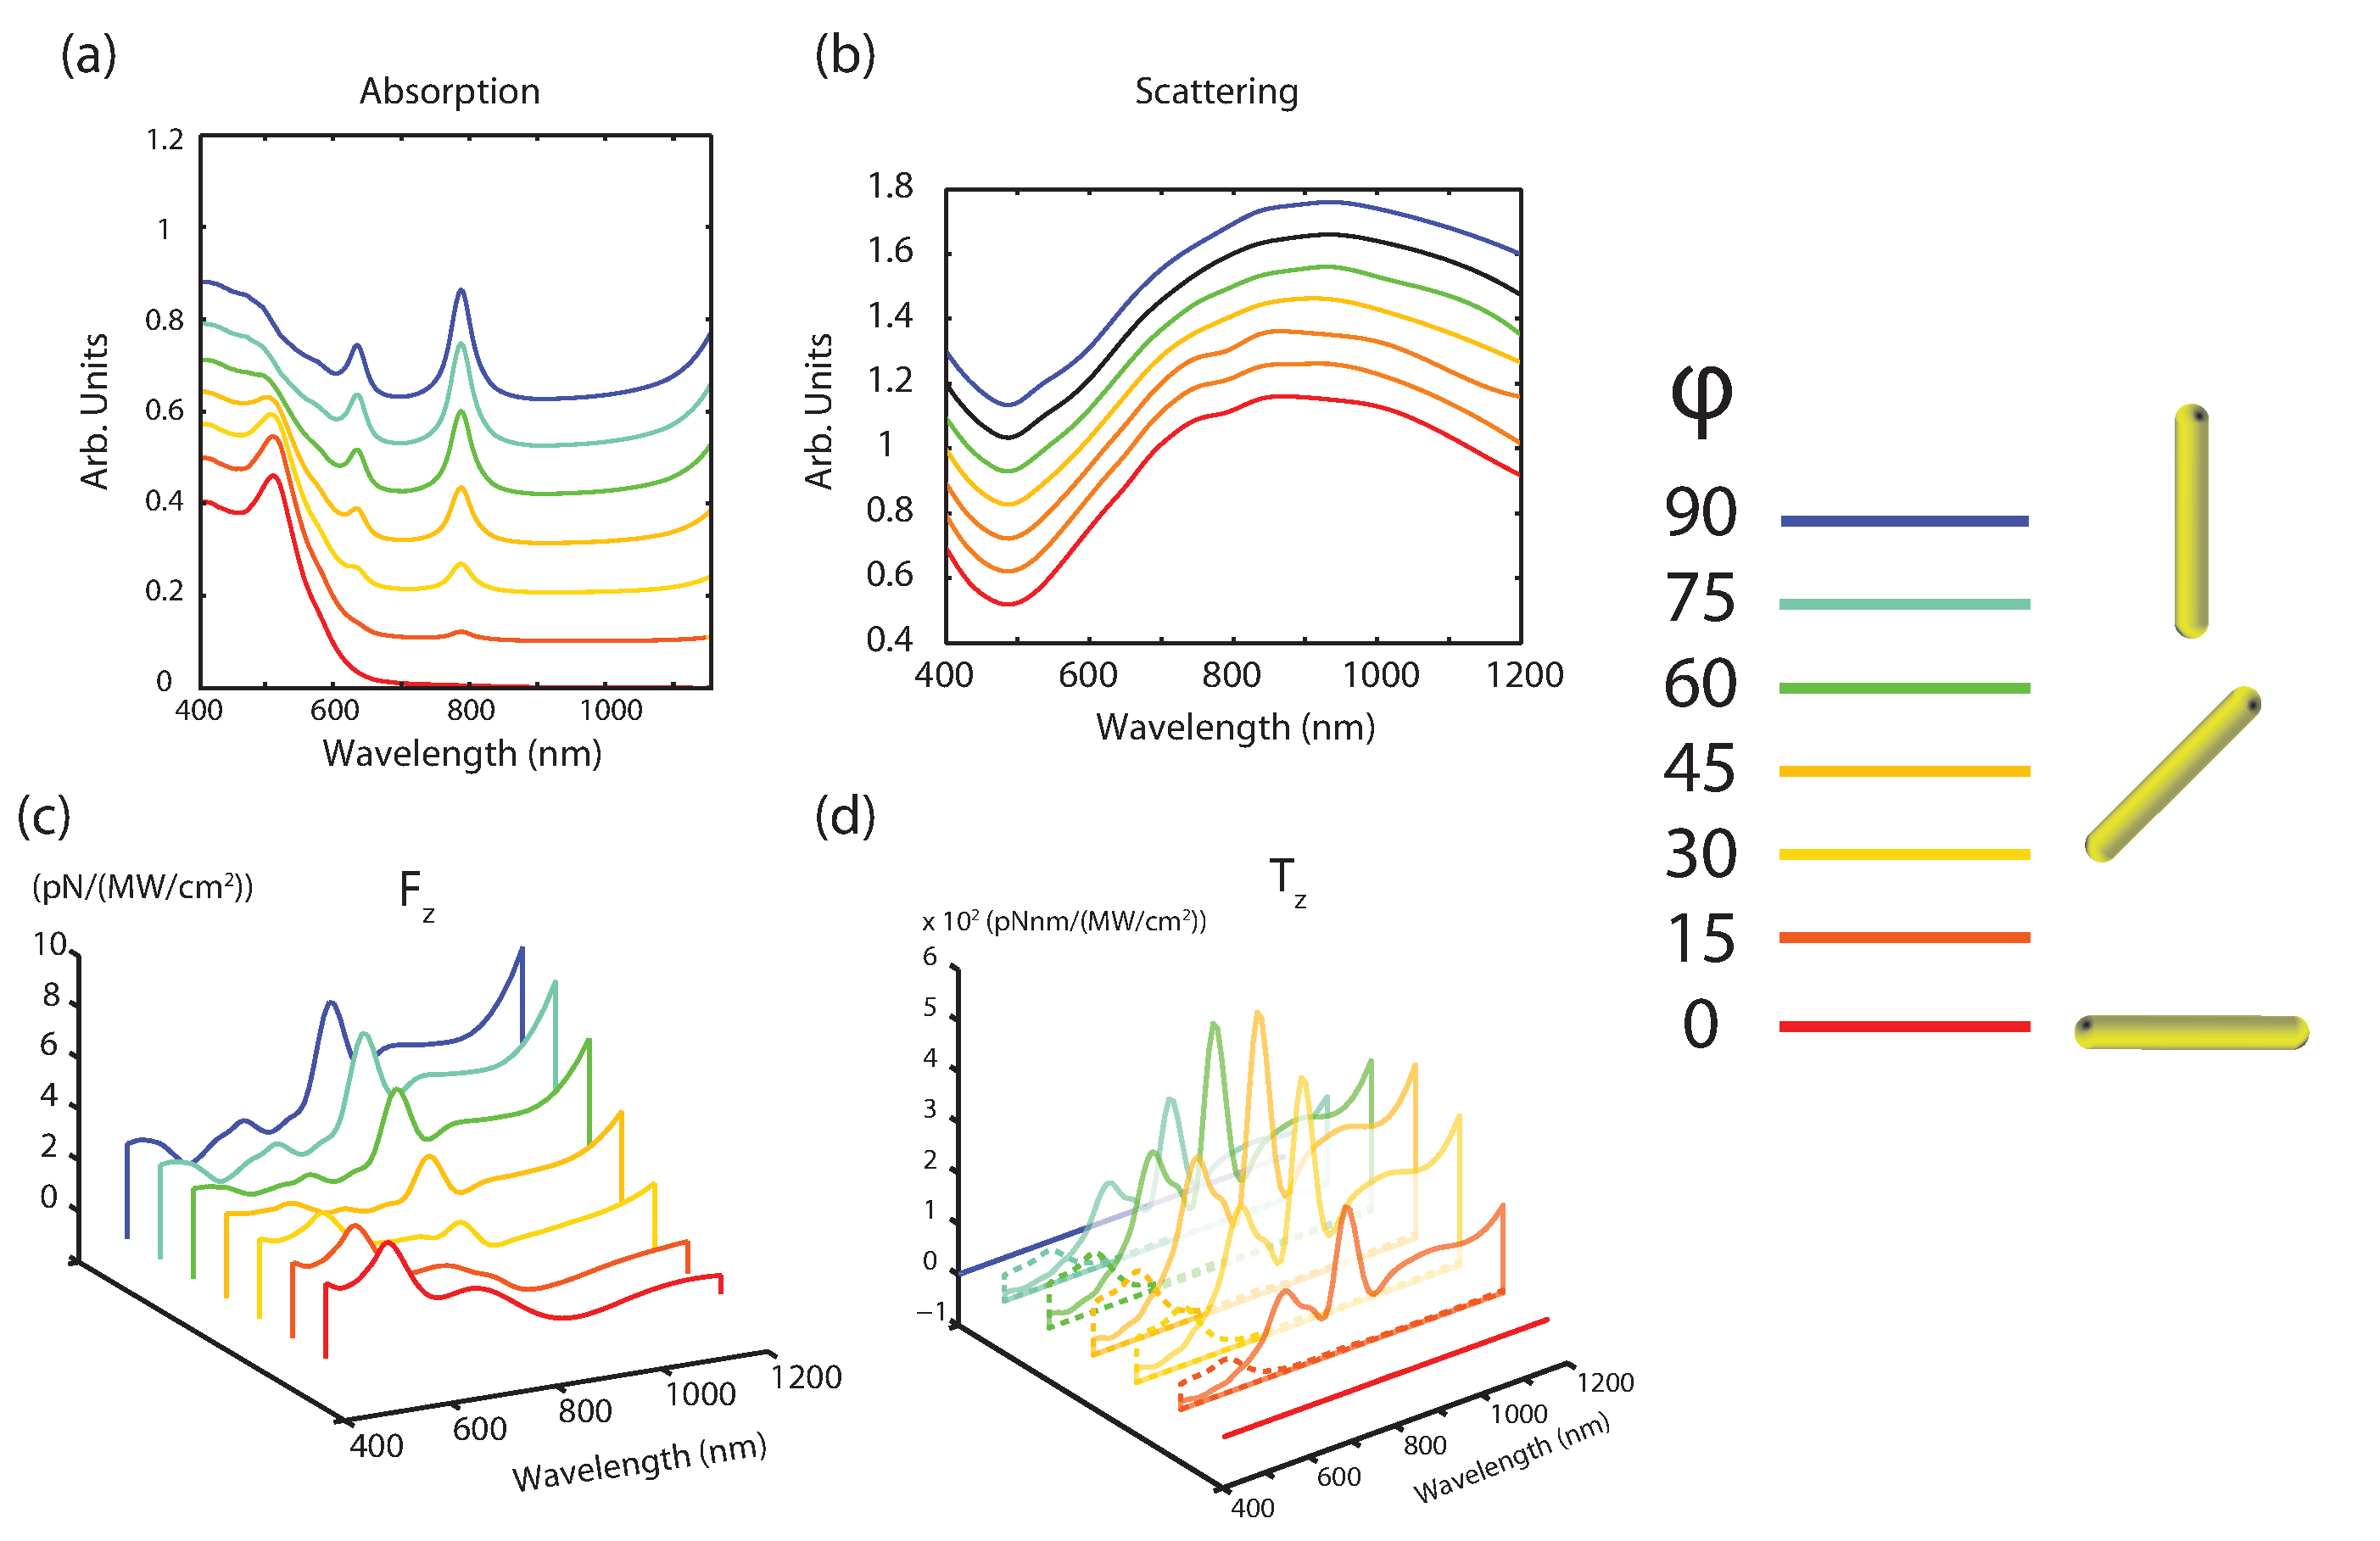
\includegraphics[width=\textwidth]{ScattAbsorptionF_zT_z.pdf}
\caption{Characteristics of a nanowire in the $x$-$y$ plane for varying orientation angle $\phi$ with $\theta = 90^\circ$. (a) Absorption cross-section. (b) Scattering cross-section, ((a), (b) spectra offset for clarity). (c) Net longitudinal force in the direction of light propagation, $-F_z$,  associated with the plasmonic Lorentz force. (d) In-plane torque $T_z$ produced by plasmons $\mathbf{f}_M$ (solid lines) and the induced electric dipole $\mathbf{f}_E$ (dashed lines).}\label{absorption}
\end{figure}

The study is introduced with a presentation of the well-studied plasmon-induced forces when the nanowire is normal to the incident electromagnetic wave, which represents the experiments performed when wires are pressed via radiation pressure along a normal surface such as a microscope slide in a 2-D trap [\cite{Tong}]. In this configuration, chiral plasmons are not produced; nevertheless, surface plasmons produce significant Lorentz forces.  Figure \ref{absorption}(a) shows the absorption cross-section for a nanowire in this transverse configuration. When the nanowire is aligned with the polarization of incident radiation ($\theta = 90^\circ, \phi = 90^\circ$), the longitudinal modes ($\lambda$ = 625nm, 790nm) are present; when it is aligned perpendicular ($\theta = 90^\circ, \phi = 0^\circ$), only the transverse mode ($\lambda$ = 510nm) is present.
% The nanowire hemispherical ends do not produce significant dispersion or shift in wavelength resonance with respect to nanowire rotation.

The longitudinal components of $\mathbf{f}_M$ are significant (on the order of pN/(MW/cm$^2$)) in the direction of light propagation ($-z$) when the transverse and longitudinal plasmonic resonances are present [Fig. \ref{absorption}(c)]. Large longitudinal forces arise between wavelengths $\lambda=$ 900-1100nm in which there is large scattering and low absorption [Fig. \ref{absorption}(a), (b)].
% At longer wavelengths, between longitudinal modes ($\lambda=$900-1100nm), the longitudinal force arising from plasmons is unexpected
When the wire is perpendicular to the light polarization ($\phi = 0^\circ$), the longitudinal force is positive and pointed in a direction {\it opposite} to the light propagation, in a manner that is reminiscent of optical tractor beams [\cite{Ruffner2012}]; when the wire is aligned parallel to the linear polarization of light ($\phi = 90^\circ$), the longitudinal force increases significantly. It has generally been assumed that radiation pressure produces the strong longitudinal forces of nanowires; that longitudinal forces are {\it also} produced via surface currents implies additional considerations and the importance of understanding plasmonic Lorentz forces.  Such plasmonic forces are strong even when there is minimal plasmonic absorption suggesting that the scattering off nanostructures plays a role.

Provided here is a comparison of the longitudinal components of $\mathbf{T}_E$ and $\mathbf{T}_M$ [Fig. \ref{absorption}(d)] which further points to the importance of plasmonically-induced Lorentz forces although the contributions are qualitatively similar in 2D.  Both torque terms are negligible when either $\phi = 0^\circ$ or $\phi = 90^\circ$ and both terms are largest at $\phi = 45^\circ$. The trends are in agreement with prior experimental results where a nanowire tends to aligns parallel or perpendicular to the illuminating polarization \cite{Tong}; however, the effect of surface plasmons is significantly larger than that associated with the electric dipole.  The underlying physical phenomena associated with nanowires is wavelength-dependent: at the transverse resonance, the in-plane rotation of nanowires is produced by the induced electric dipole force $\mathbf{f}_E$.  At longer wavelengths, it is the rotation induced by surface plasmons via Lorentz forces $\mathbf{f}_M$ that dominates.  This is a central conclusion of this chapter: plasmonically-induced Lorentz forces are significant at longer wavelengths and are often stronger than electric-dipole induced forces, even when there is minimal absorption due to plasmon excitation.

\section{Translation and compressive plasmonic forces}\label{forces}
\subsection{Force visualized for various illumination wavelengths}
\begin{figure}[ht]
\centering\includegraphics[width = \textwidth]{fig4.pdf}
\caption{Forces on the nanowire surface produced by the surface currents (red arrows) and the norm of the surface magnetic field (surface colormap) for oblique geometries that excite the chiral hybrid plasmonic mode, where (a) $\theta = 15^\circ, \phi = 90^\circ$ (b) $\theta = 30^\circ, \phi = 75^\circ$ (c) $\theta = 60^\circ, \phi = 60^\circ$ at $\lambda = 1071$nm.}\label{wireforce}
\end{figure}

A graphical representation of the forces produced by plasmons $\mathbf{f}_M$ on three oblique geometries are illustrated with arrows in Fig. \ref{wireforce} for illuminating wavelength $\lambda = 1071$nm. The chiral-hybrid plasmons result from a superposition of the three lowest order modes ($|m|\leq 1$) [Eq. \ref{Efield}]. The nanowire surface color denotes the relative strength of the time-averaged magnetic field.  Chiral helices are also visible in the electric field. Both on and off resonance, the Lorentz forces yield compression forces on the nanowire.  While the Lorentz forces are generally directed into and towards the axis of the nanowire, it varies in magnitude along the surface of the nanowire. In oblique illumination geometries ($\theta \neq 0^\circ$ or $90^\circ$), the magnetic-field and plasmonic Lorentz force patterns are not symmetric across the length or width of the wire. This break in azimuthal and longitudinal symmetry subsequently yields net forces in the $x, y, z$ direction that would result in translation and torque of the nanowire. The origin of the asymmetrical profile along the length of the nanowire stems from the lossy nature of the material, plasmons are coupled into the nanowire via the termination and propagate the length of the nanowire, which acts like a low-Q Fabry-P\'{e}rot resonator [\cite{Ditlbacher}]. The remaining part of this section describes the volume-integrated net translation forces; Sec. \ref{3D} will discuss the net torque of the nanowires.

Figure \ref{FxFyFz} illustrates $\mathbf{f}_M$ for $0<\theta<$ 90$^\circ$ and $0<\phi< $90$^\circ$. From this quarter-hemisphere, all nanowire positions are deduced.  Five wavelengths are shown, which are uniformly spaced in the frequency domain.  A wavelength below the transverse resonance ($\lambda =$ 441nm) is illustrated, wavelengths associated with the transverse (HE$_{\pm 1}$) and longitudinal (TM$_0$) modes ($\lambda =$ 517, 625, and 790nm), and a longer, off-resonance wavelength associated with the hybrid chiral plasmon ($\lambda =$ 1071nm).  The orientations and wavelengths that correspond to Fig. \ref{wireforce} are marked.  The color mappings are symmetrized; the components of $\mathbf{f}_M$ are both positive and negative.

\begin{figure}[t!]
\centering\includegraphics[width = \textwidth]{AllF.png}
\caption{Net (volume-integrated) Lorentz forces associated with nanowire surface currents $\mathbf{f}_M$ in (a) $x$-direction, (b) $y$-direction, and (c) $z$-directions for illuminating wavelengths $\lambda = $ (i) 441nm (ii) 517nm (iii) 625nm (iv) 790nm (v) 1071nm.}\label{FxFyFz}
\end{figure}

Plasmons on the nanowire not only yield longitudinal forces [Fig. \ref{absorption}(c)] but also appreciable forces {\it perpendicular} to the light Poynting at wavelengths where there is lower absorption and higher scattering.  In general, the largest net translation forces are produced in the $y$-direction or direction of light polarization.  The force perpendicular to the polarization, that is, in the $x$-direction, is negative at lower wavelengths, but either positive or negative at longer wavelengths, depending on the alignment of the wire.  Moreover, the net translation forces are small on resonance compared to at longer wavelengths where chiral plasmons are present.  For example, at the transverse and longitudinal resonances, that is, $\lambda = 510$nm and $\lambda = 790$nm, the net translation forces are at most 2pN/(MW/cm$^2$), whereas at the wavelength of $\lambda = 1071$nm, the net translation force is as much as 15pN/(MW/cm$^2$). Therefore, the Lorentz forces that occur via scattering transfer momentum to the nanowire in a manner that does not require strong plasmonic absorption since there is large scattering [Fig. \ref{absorption}(b)] yet low absorption [Fig. \ref{absorption}(a)] where Lorentz forces are greatest.

\begin{figure}[!t]
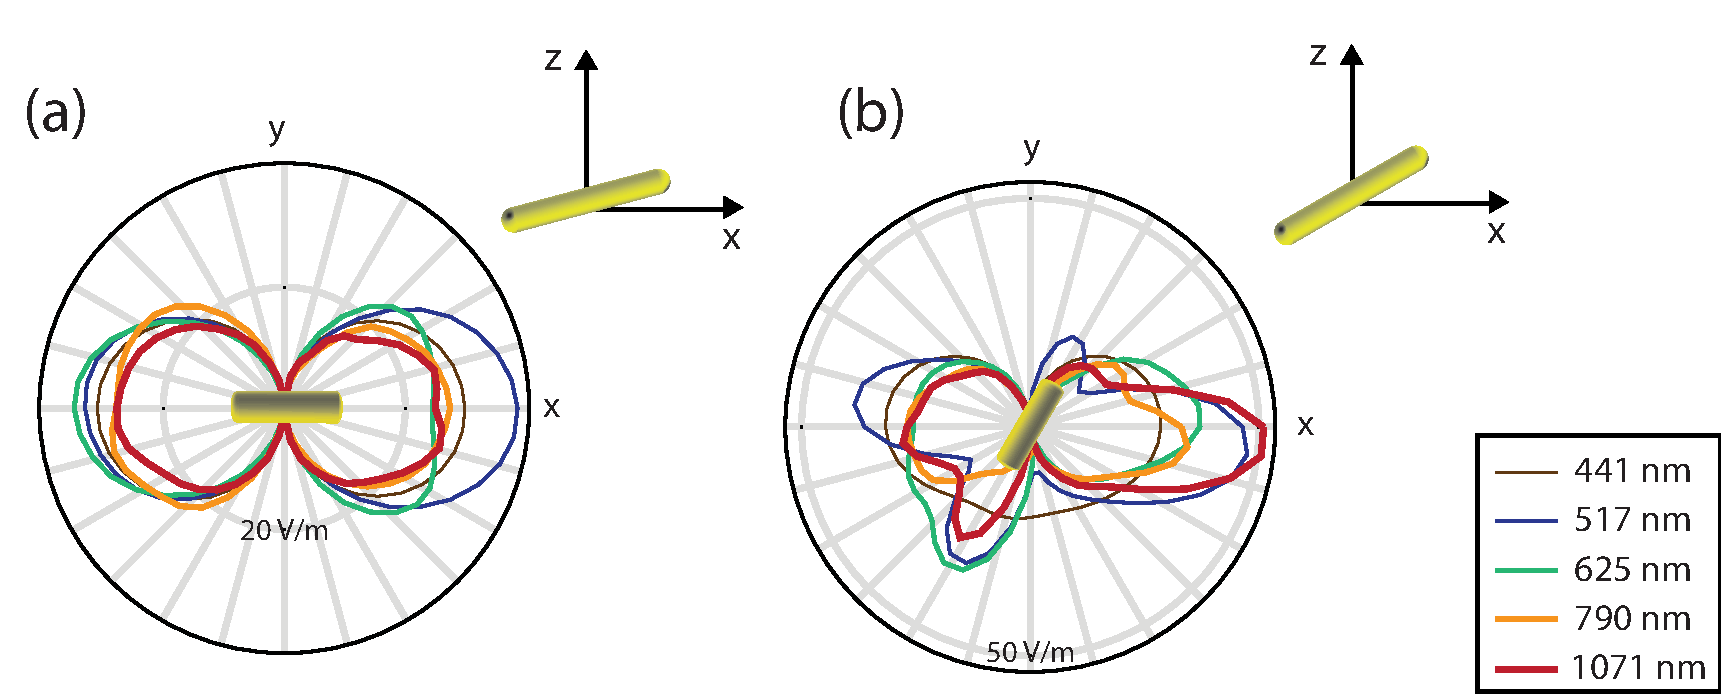
\includegraphics[width = 1.0\textwidth]{CPLComp.pdf}
\caption{Far-field radiation patterns for a nanowire aligned (a) in the $x$-$z$ plane with $\theta$ =75$^\circ, \phi$ = 0$^\circ$, (b) $\theta$ = 60$^\circ$, $\phi$ = 60$^\circ$ for wavelengths $\lambda$ = 441nm, 517nm, 625nm, 790nm, and 1071nm.}\label{CPLComp}
\end{figure}
\subsection{Momentum transfer via scattering}
It is expected that momentum transfer in the transverse $x$-$y$ plane associated with plasmons is observable in the scattered fields in order for linear momentum to be conserved and simulations indicate that momentum conservation is visible in the far-field power.
%The scattering of light is synonymous with the excitation of plasmons and thus a good indication of the plasmon dynamics.
Figure \ref{CPLComp} shows the electric field norm in the far field for two geometries to illustrate transverse forces, from which the scattering dynamics can be extrapolated. The momentum transfer to the nanowire can be inferred by the symmetry of the dipole  radiation patterns.  In Fig. \ref{CPLComp}(a), the nanowire is aligned in the $x$-$z$ plane with $\theta = 75^\circ$ and $\phi=0^\circ$.  At this orientation, the Lorentz force is calculated in the $x$-direction to be either negative ($\lambda =$ 441, 517nm) or positive ($\lambda =$ 625, 790, 1071nm) depending on the illuminating wavelength [Fig. \ref{FxFyFz}(a)].  A positive value of $F_x$, at a wavelength of $\lambda =$ 441nm is largely attributed to reflection since this wavelength is below the transverse-resonance cutoff.  At higher wavelengths, the $x$-direction shifts in the far-field radiated power correspond with the sign of the plasmonic Lorentz forces in the $x$-direction. The shape of the far-field radiation corresponds to the characteristic dipole radiation from excitation of the longitudinal TM$_0$ mode.

Similarly, in Fig. \ref{CPLComp}(b) shows a similar far-field normalized power for geometry $\theta$ = 60$^\circ$ and $\phi$ = 60$^\circ$.  Below the cutoff for plasmon excitation ($\lambda$ = 441nm), the radiation pattern indicates that momentum transfer in the $y$-direction is due to reflection. At higher wavelengths, an ``antenna'' behavior of the wire is apparent, the radiation pattern exhibits directionality.
% We observe that the wire radiates as an oscillating electric dipole in its transverse plane in addition to in the $y$-direction due to excitation of the transverse mode.
 The dipole radiation mode in the $y$-direction and transverse modes are uncoupled at $\lambda$ = 517nm, and the far-field radiation pattern is an `$x$' shape that is aligned with the axis of the nanowire. The size of the arms of the `$x$' shape determine the relative strengths of the dipole modes present, the arm perpendicular to the nanowire axis corresponds to the fundamental, TM$_0$ mode and the arm parallel to the HE$_{\pm1}$ modes.

At longer wavelengths the plasmonic Lorentz forces are significant [Fig. \ref{FxFyFz}]. For wavelengths and orientations that produce significant Lorentz forces the far-field radiation patterns differ greatly in symmetry from dipole radiation patterns one might expect. For wavelengths of $\lambda = 625, 790,$ and $1071$nm, the center of radiation pattern moves in the positive $x$ and negative $y$-direction, corresponding with $\mathbf{f}_M$ that is negative in the $x$ and positive in the $y$-directions [Fig. \ref{FxFyFz}].
%The scattering of light points to new self-action effects, which, in addition to reflection and radiation pressure, are observed in the far-field radiation power patterns.
Figure \ref{CPLComp} indicates that the plasmonically-induced Lorentz forces result in 50-70$\%$ changes in far-field radiated power, which is experimentally measurable.


\section{Torque in 3-dimensions}\label{3D}
\subsection{Torque visualized for various illumination wavelengths}
\begin{figure}[b]
\centering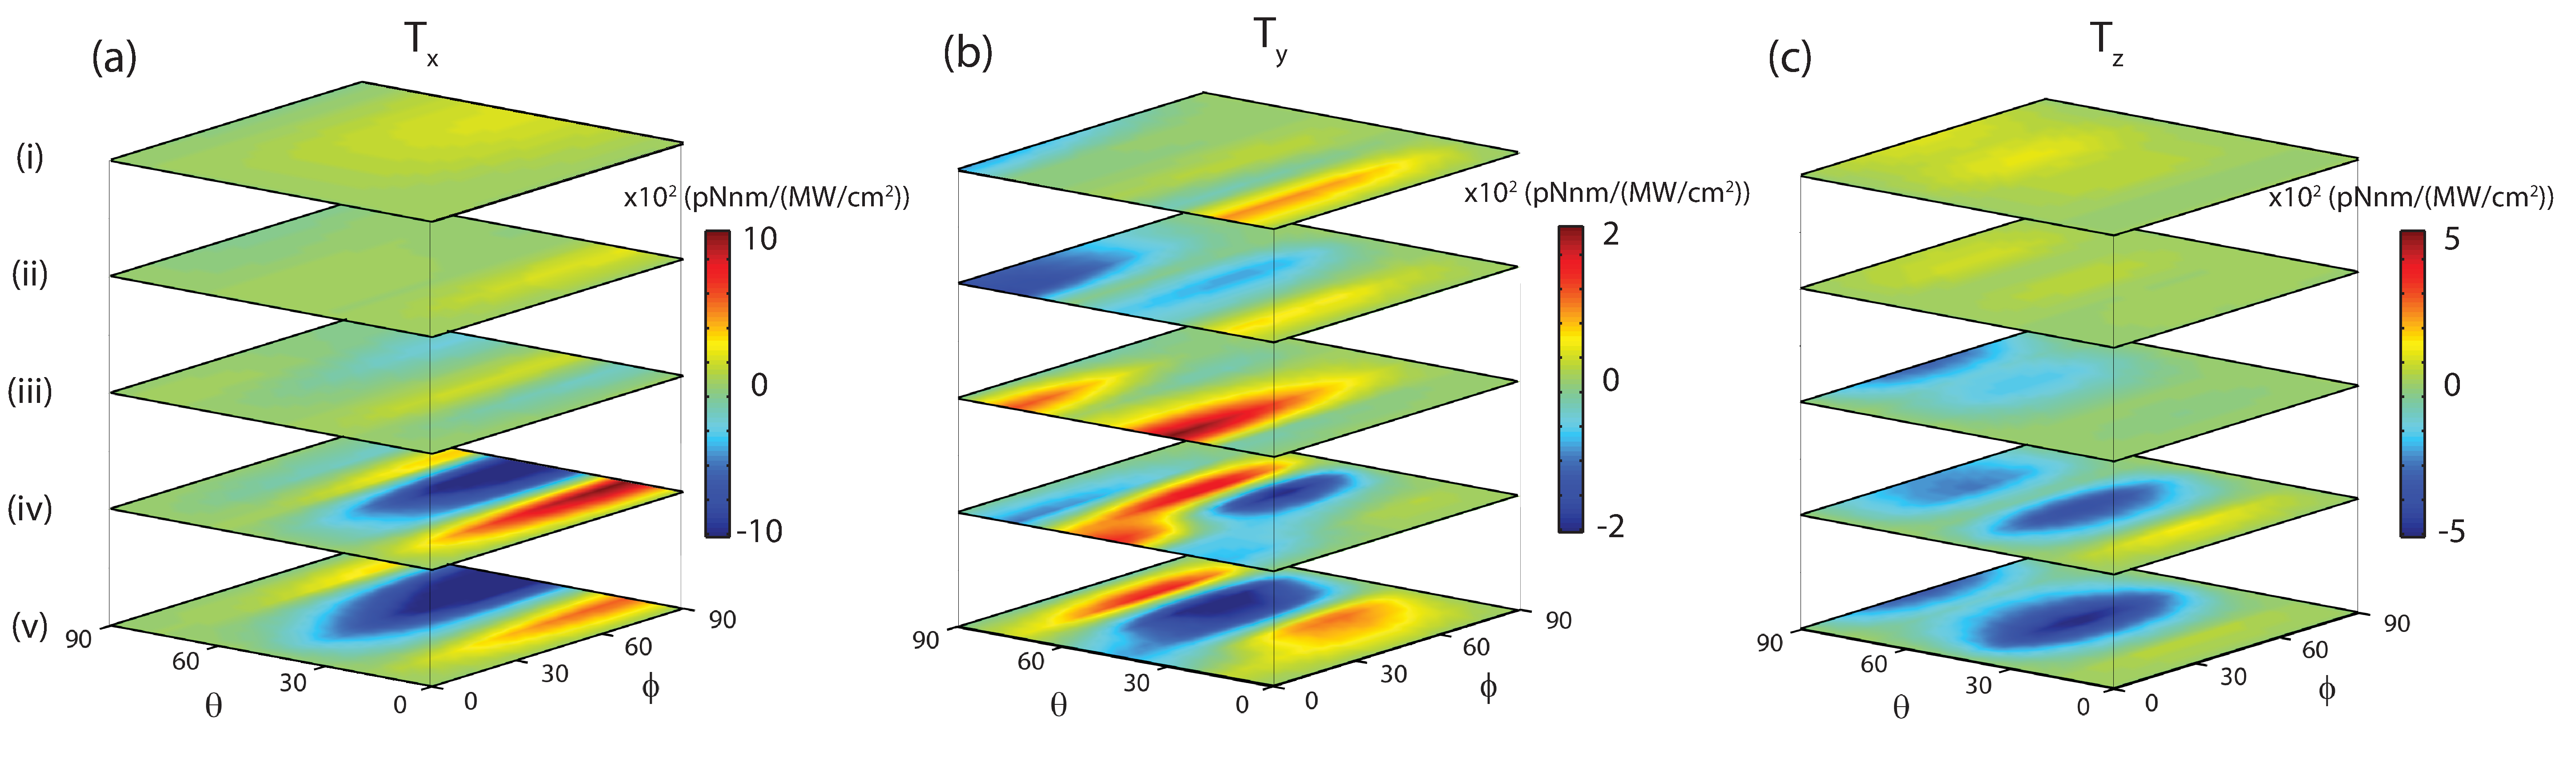
\includegraphics[width = \textwidth]{TNMT.pdf}
\caption{Torque around the (a) $x$-axis, (b) $y$-axis, and (c) $z$-axis at (i) 441nm, (ii) 535nm, (iii) 625nm, (iv) 790nm, and (v) 1071nm.}\label{TNW}
\end{figure}


The vector components of the dipole moment and plasmonically-induced Lorentz torque [$\mathbf{T}_E +\mathbf{T}_M = (T_x,T_y,T_z)$] are shown in Fig. \ref{TNW} for five wavelengths (441, 517, 625, 790, and 1071nm as chosen in the previous section).  Large values of $T_x$ and $T_z$ represent large torques that rotate the nanowire in both the polar and azimuthal directions. $T_x$ and $T_z$ increase in magnitude as wavelength increases which correlates well to the existence of chiral hybrid modes at longer wavelengths. Subsequently, whether $T_x$ and $T_y$ are positive or negative depends on the polar orientation of the nanowire.

The orientations that produce large net translation forces [Fig. \ref{FxFyFz}] do not necessarily coincide with large torques [Fig. \ref{TNW}]; the greater the asymmetry in $\mathbf{f}_E$ and $\mathbf{f}_M$, the greater the torque. Maximal torques produced by plasmons ($\mathbf{T}_M$) are an order of magnitude larger than the maximal torques produced by dipole moments ($\mathbf{T}_E$). Moreover, the magnitude of $\mathbf{T}_E$ is negligible at wavelengths above 600nm; above 600nm, $\mathbf{T}_M$ dominates. The magnitude of the $\mathbf{T}_E$ is the same sign in our hemisphere quadrant of $\theta$ and $\phi$ since $\mathbf{f}_E$ uniformly aligns the induced dipole with the axis of field polarization. In contrast, $\mathbf{T}_M$ changes sign with nanowire orientation and illuminating wavelength [Fig.~\ref{TNW}], which reflects the sensitive nature of the chiral hybrid plasmon.

\subsection{Phase diagram illustrations}
When the nanowire is free to rotate in three dimensions, the rotational behavior becomes complicated. The torque on the nanowire causes rotation which subsequently changes the torque on the nanowire. The results of this system that only accounts for Lorentz forces yields nonlinear dynamics that are beyond the scope of this chapter; nonetheless, the dynamics are illustrated with a phase portrait of the torques in spherical coordinates. The rotation in the $\theta$ and $\phi$ directions associated with $\mathbf{T}_E$  + $\mathbf{T}_M$ are:
\begin{eqnarray}
A_{\theta} &=& -\sin\phi T_x + \cos\phi T_y \label{Atheta}
\\A_\phi &=& T_z. \label{Aphi}
\end{eqnarray}

\begin{figure}[!ht]
\centering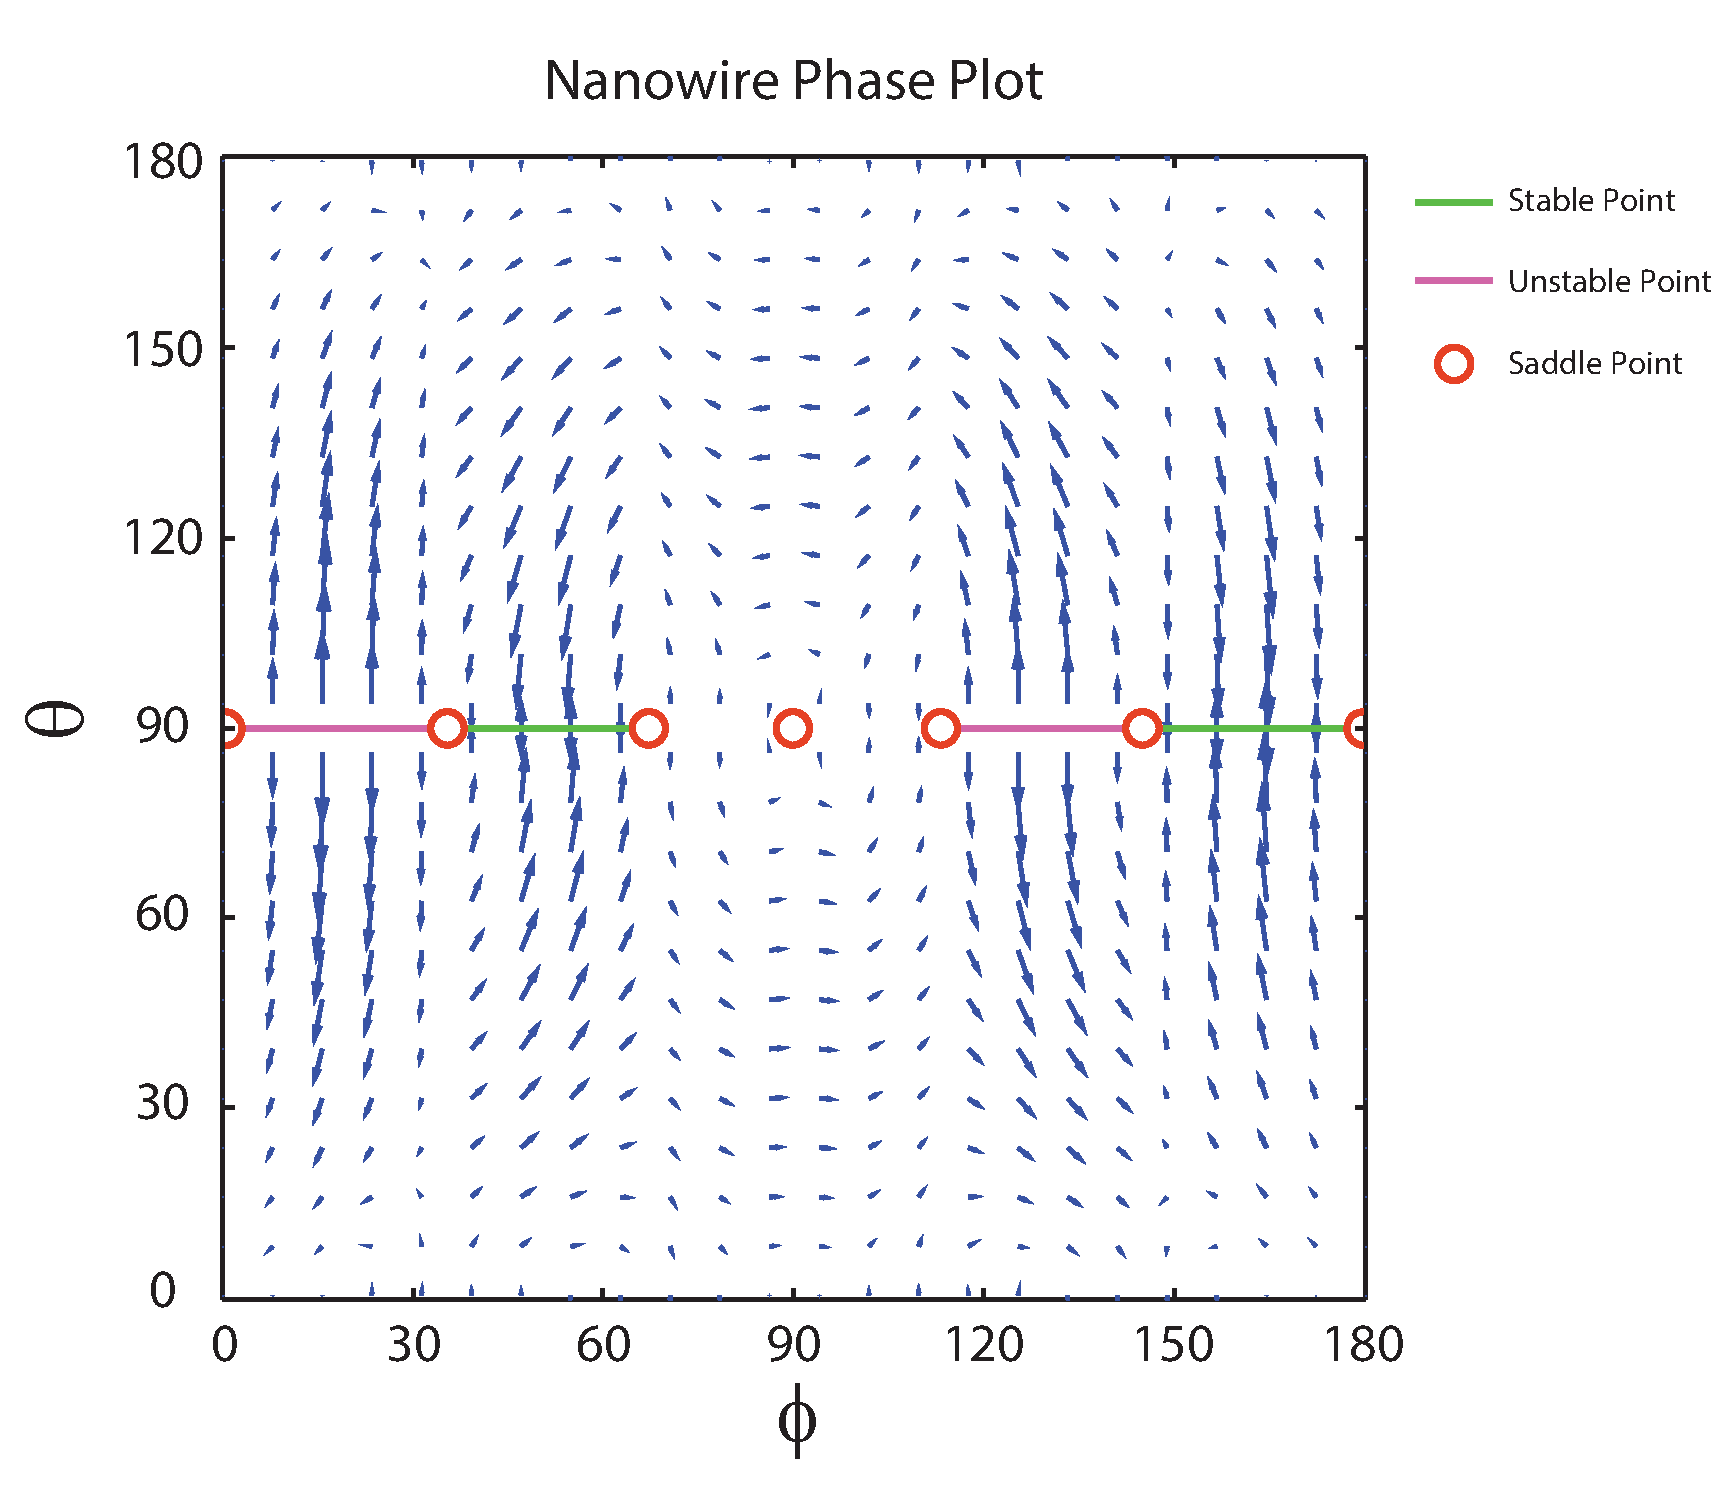
\includegraphics[width = \textwidth]{Rotational_Torque_1071nm.pdf}
\caption{Phase portrait of the torque forces calculated at $\lambda$ = 1071nm. Arrows in the $x$ and $y$ directions indicate torque that rotates the nanowire in the $\phi$ and $\theta$ directions respectively.}\label{RotTorq1071}
\end{figure}
The phase portrait, i.e. vectors $[A_{\phi},A_{\theta}]$ as a function of $\theta$, $\phi$ of the nanowire are plot in Fig. \ref{RotTorq1071}.
$A_{\theta}$ and $A_{\phi}$ are not equivalent to the angular acceleration since the rotational inertia, which changes as a function of angle, has not been taken into consideration. Moreover, the angular velocity will also influence the angular acceleration when the rotational inertia changes. Nonetheless, an understanding is gathered of the nanowire's stable orientations and dynamics from Fig. \ref{RotTorq1071}.

Points of stability occur when the angular motion is zero, which occurs when the torque is zero. Stable points occur when the vector field flows toward the point of zero torque; unstable points occur when the vector field flows away from the point of zero torque [\cite{Strogatz}]. Saddle points occur when the vector field flows toward the point of zero torque in one direction, and away in another.


Similar to the observation of the 2D nanowire dynamics [Sec. \ref{intro}], the nanowire aligns either parallel or perpendicular to the axis of polarization in a 3D system, settling at a stable point. Stable points occur when either $\theta$ or $\phi$ are equal to 0$^\circ$ or 180$^\circ$, and $\theta$ = 90$^\circ$ consistent with the strong orientational trapping observed in previous research [\cite{Yan2012a,Tong}]. Interestingly, along the line of $\theta$ = 90$^\circ$ stable, unstable and saddle points exist and illustrate many rich and complicated dynamics already reported with the optical trapping of nanowires. Around stable fixed points oscillatory dynamics occur: the nanowire will rotate, but more specifically, it will rock and spin in an oscillatory manner. Fig. \ref{RotTorq1071} also explains the rotational accelerations and rapid reversals seen in light-driven experiments [\cite{Shelton2005}] that are associated with the saddle point behavior and sharp inflections, such as those dynamics indicated at $\theta$ = 90$^\circ$.

This alludes to competing dynamics between the induced electric dipole and surface plasmons and explains the prior experimental observations that often contradict. It has been previously reported that nanowires align parallel or perpendicular to the linearly polarization of an optical trap. A theoretical model that limits consideration to $\mathbf{T}_E$ only explains the stable alignment of the dipole parallel to the polarization. Yet moreover, prior experiments employ trapping wavelengths in the near-IR [\cite{Tong}], where the magnitude of $\mathbf{T}_E$ is predicted to be negligible. This model predicts and explains the stable orientations of the nanowire, with longitudinal axis both parallel and perpendicular to the field polarization.

\section{Conclusion} \label{conclusion}
This chapter has shown that plasmonically-induced Lorentz forces are significant and greater than dipole-moment-induced forces, particularly at long-wavelength excitation between plasmon resonances.  The nanowire forces produced by plasmons lead to axial compression, which changes spatially along the nanowire surface depending on the nanowire orientation.  The existence of chiral plasmons coincides with spiral magnetic-field patterns that produce net transverse forces and torques, which is predicted to be experimentally observable in the far-field radiated power and polarization.  The plasmonically-induced Lorentz forces are expected to interfere with the optical trapping of nanowires; selection of a laser-trap wavelength that prevents the excitation of the chiral plasmonic modes will enable greater control over the optical manipulation of nanowires.

The rotational dynamics present a highly nonlinear and complicated problem due to the sensitive nature of the plasmonic resonance that conventional ray optics cannot explain. The plasmonically-induced Lorentz forces and torques produce rotational motion consistent with the spinning, rocking, and rapid reversals in rotation observed experimentally with elongated plasmonic nanoparticles.  Plasmonically-induced torque may oppose the dipole-induced torque, although the Lorentz torque dominates almost completely above the transverse resonance of the nanowire. This theoretical investigation is the first to properly explain the stable positions of nanowires under illumination of linearly-polarized electromagnetic fields, and reveals a rich system of optomechanical plasmonically driven dynamics that has not yet been explored.

This work also points to novel methods that manipulate conducting nanoparticles that do not result in the extreme absorption and heating generally associated with the excitation of plasmons; strong plasmonically-induced Lorentz forces occur off-resonance where plasmonic absorption is minimal. This outcome is highly relevant to the development of new devices and mechanisms that efficiently leverage the nonlinear mechanical dynamics of conducting nanoparticles in fluids, not limited to elongated conducting particles but also chiral nanoparticles, polymer materials, and carbon metastructures.

\section{Future work}
Future work on this subject may involve experimental verification of the theoretical and numerical components of the work shown here. An experiment may consist of an microscope setup with two tightly focused beams at different wavelengths. One beam would act as the optical trapping beam that would stabilize the nanowire at the focal point of the microscope setup similar to the setups described in the references [\cite{Ashkin2001, Lee2012, Kuo2001, Lang2003}], and the other would act as the excitation beam that would generate the Lorentz forces described in this chapter.